
\subsection{Prototypische Implementierung des Anwendungsfalls}
Angewandtes/angepasstes System-Modell
pro Schritt benutztes Sicherheitstechnologie erklären/erwähnen

im Modell auch Schnittstellen, z.B. für SAP Integration, HANA, Leonardo Blockchain und Machine Learning, um zu verdeutlichen, dass die Anforderungen zur sowohl vertikalen (SAP Integration) und horizontalen (Blockchain) erfüllt werden können

\subsubsection{Anbindung der Sensoren an das Edge-Gerät}

\begin{figure}
  \centering
  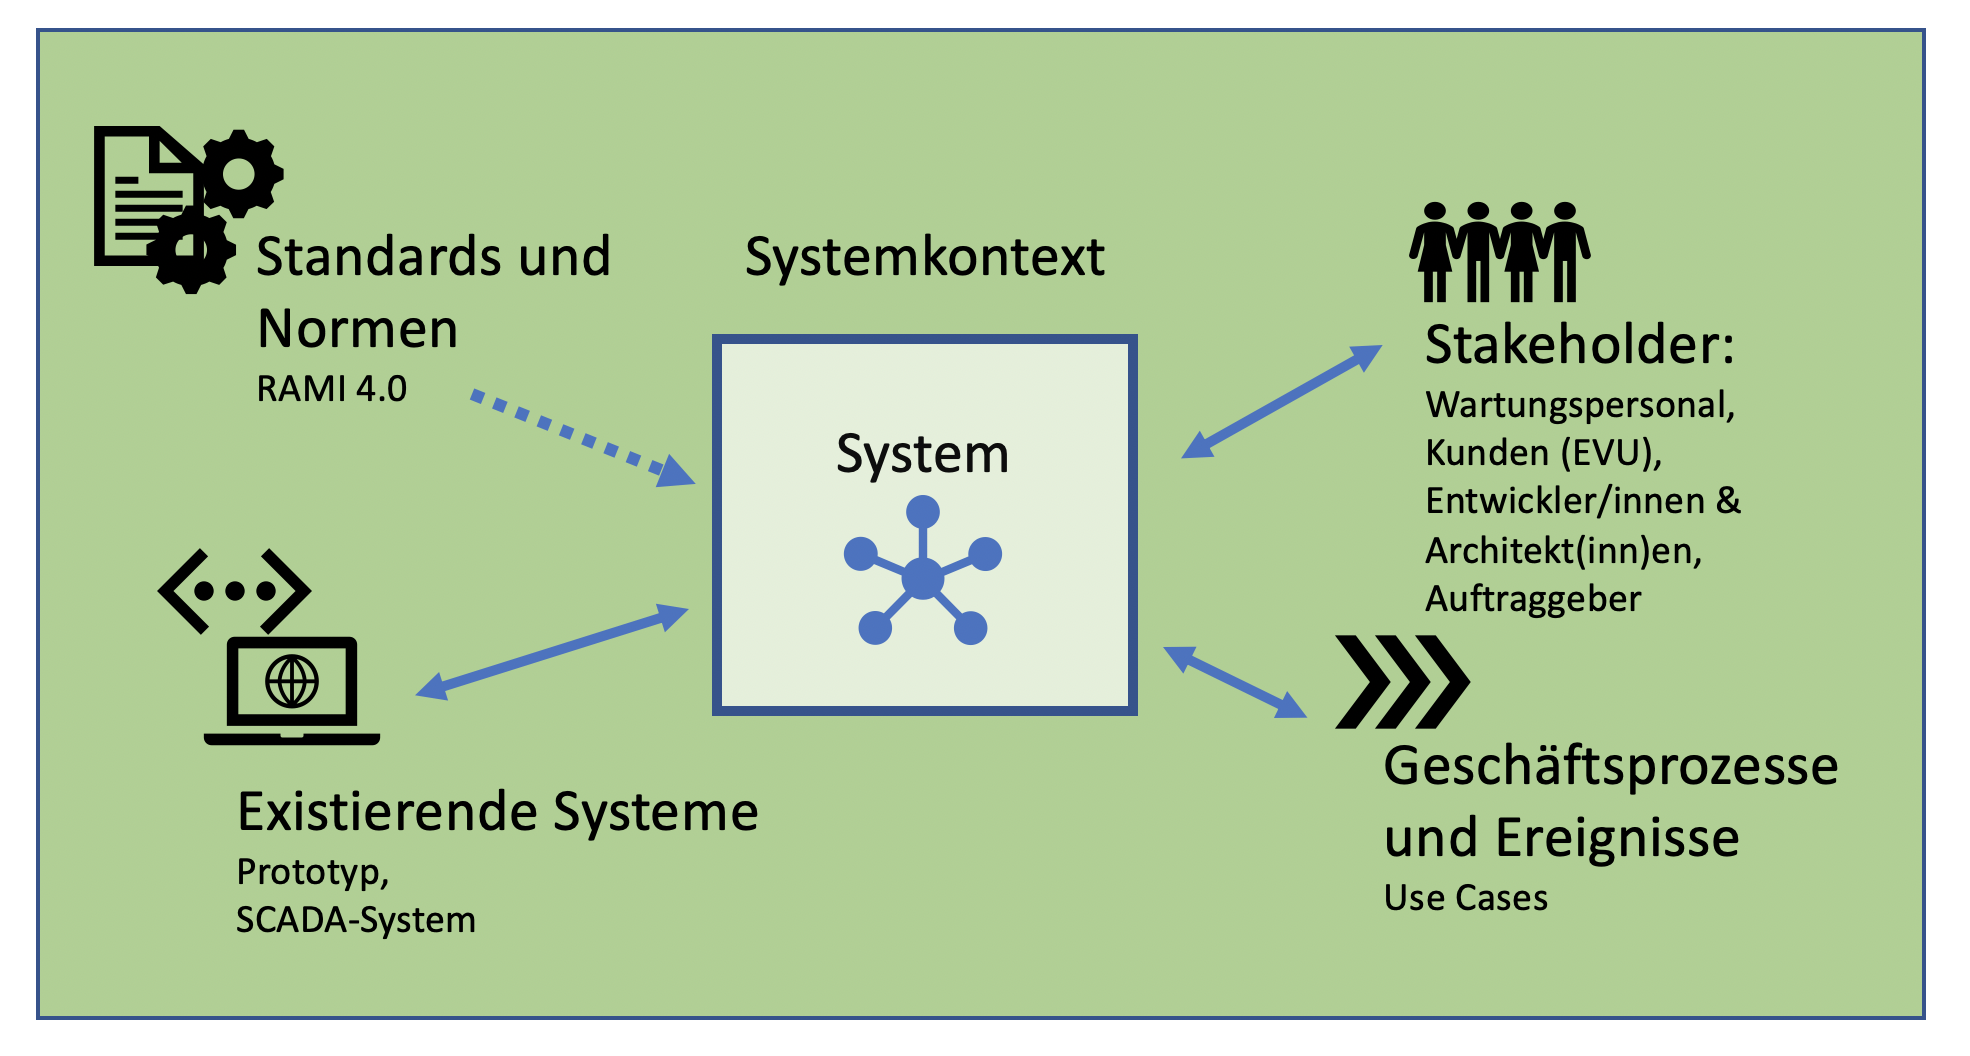
\includegraphics[width=1\linewidth]{System_Kontext.png}
  \caption[Systemabgrenzung und Systemkontext]{Systemabgrenzung und Systemkontext}
  \label{kontext}
\end{figure}

\subsubsection{Geräteverwaltung}
mit SAP Cloud Platform Internet of Things und Device Model hier erstellen und als Bild einfügen und außerdem
zunächst auf Tenants und User eingehen und Einrichtungs des Services generell erklären mit eventuell den Message Processings
und Gateways etc

\subsubsection{Einrichtung der Gateway-Edge}

\begin{lstlisting}
  {
  "id": "2019161729",
  "alternateId": "1122334455667788",
  "protocolId": "rest",
  "name": "IoT Gateway REST",
  "type": "edge",
  "creationTimestamp": 1571741372988,
  "status": "online",
  "version": "4.42.0",
  "operatingSystem": "Linux;4.19.75-v7+;arm"
}

\end{lstlisting}


\subsubsection{Senden der Daten an die Cloud}

\begin{lstlisting}
============================================
Reading sensor data ...
{'capabilityAlternateId': '1234', 'measures': [{'temperature': '19.0'}, {'wind_speed': '1.12102078977'}, {'pressure': '1010'}, {'humidity': '70.0'}, {'airtight': '1.2'}], 'sensorAlternateId': '1234'}
==> HTTP Response: 202
\end{lstlisting}

\subsubsection{Erstellen des digitalen Zwillings}

\paragraph{Events}

\subsubsection{Visualisierung mit einer UI5-Applikation}

\subsubsection{Benachrichtigung mit AWS SNS-Server}

\subsubsection{Events generieren mit NodeJs}

\subsubsection{Zusammenfassung Implementierung}

\newpage
